\documentclass[10pt]{article}
 
\usepackage[margin=1in]{geometry} 
\usepackage{amsmath,amsthm,amssymb, graphicx, multicol, array}
\usepackage{statex2} % for uniform dist. symbol
 
\pagecolor{white} % make page white

\renewcommand{\qedsymbol}{} % remove qed symbol
 
\newenvironment{problem}[2][Problem]{\begin{trivlist}
\item[\hskip \labelsep {\bfseries #1}\hskip \labelsep {\bfseries #2.}]}{\end{trivlist}}

 \usepackage{enumitem}

\begin{document}
 
\title{Problem Set: Continuous Random Variables}
\author{James Heald\\
Gatsby Bridging Programme 2023}
\date{}
\maketitle

\begin{problem}{1}
Suppose $X$ is a continuous random variable whose probability density function is given by
\begin{align*}
    f_X(x) &= 
    \begin{cases}
      C(4x-2x^2) & \text{if}\ 0 < x < 2 \\
      0 & \text{otherwise.}
    \end{cases}
\end{align*}
\begin{enumerate}[label=(\alph*)]
\item What is the value of $C$? 
\item Find $P(X > 1)$.
\end{enumerate}
\end{problem}

\begin{problem}{2}
The amount of time in hours that a computer functions before breaking down is a
continuous random variable with probability density function given by
\begin{align*}
    f_X(x) &= 
    \begin{cases}
      \lambda e^{-x/100} & \text{if}\ x \geq 0 \\
      0 & \text{if}\ x < 0.\\
    \end{cases}
\end{align*}
What is the probability that
\begin{enumerate}[label=(\alph*)]
\item a computer will function between 50 and 150 hours before breaking down?
\item it will function for fewer than 100 hours?
\end{enumerate}
\end{problem}
 
\begin{problem}{3}
Buses arrive at a specified stop at 15-minute intervals starting at 7 A.M. That is, they
arrive at 7, 7:15, 7:30, 7:45, and so on. If a passenger arrives at the stop at a time that
is uniformly distributed between 7 and 7:30, find the probability that they wait
\begin{enumerate}[label=(\alph*)]
\item less than 5 minutes for a bus;
\item more than 10 minutes for a bus.
\end{enumerate}
\end{problem}

%\begin{problem}{1}
%%For the probability density function given by
%The distribution of the amount of gravel (in tons) sold by a company in a week has a probability density function given by
%\begin{align*}
%    f_X(x) &= 
%    \begin{cases}
%      \frac{3}{2}(1-x^2) & \text{if}\ 0 \leq x \leq 1 \\
%      0 & \text{otherwise.}
%    \end{cases}
%\end{align*}
%With respect to this distribution, find
%\begin{enumerate}[label=(\alph*)]
%\item the 40th percentile;
%\item the median.
%\end{enumerate}
%\end{problem}
%
%\begin{proof}[Solution]
%(a) The $(100p)$th percentile is the value of $\eta(p)$ that satifies $ \int^{\eta(p)}_{-\infty} f_X(x)dx = p$.
%\begin{align*}
%\int^{\eta(p)}_0 \frac{3}{2}(1-x^2) dx &= p\\
%\frac{3}{2} \bigg[x - \frac{x^3}{3}\bigg] \bigg|_0^{\eta(p)} &= p,
% \end{align*}
% and hence $n(p) = $. Hence (a) $n(0.4) = $, and (b) $n(0.5) = $.
%\end{proof}

\begin{problem}{4}
In commuting to work, a professor must first get on a bus near her house and then transfer to a second bus. If the waiting time (in minutes) at each stop has a uniform distribution on the interval $[a,b]$, then it can be shown that the total waiting time X has the probability density function
\begin{align*}
    f_X(x) &= 
    \begin{cases}
      \frac{x}{25} & \text{if}\ 0 \leq x < 5 \\
      \frac{2}{5} -\frac{x}{25} & \text{if}\ 5 \leq x \leq 10 \\
      0 & \text{otherwise.}
    \end{cases}
\end{align*}
\begin{enumerate}[label=(\alph*)]
\item Obtain an expression for the $(100p)$th percentile $\eta(p)$ [Hint: consider $0 \leq \eta(p) < 5$ and $5 \leq \eta(p) \leq 10$ separately].
\item Find the median.
\end{enumerate}
\end{problem}

\begin{problem}{5}
The probability density function of a continuous random variable $X$ is given by
\begin{align*}
    f_X(x) &= 
    \begin{cases}
      1 & \text{if}\ 0 \leq x \leq 1 \\
      0 & \text{otherwise.}
    \end{cases}
\end{align*}
Find $\mathbb{E}[e^X]$.
\end{problem}

\begin{problem}{6}
Suppose the probability density function of the magnitude $X$ of a dynamic load on a bridge (in Newtons) is
\begin{align*}
    f_X(x) &= 
    \begin{cases}
      \frac{3x}{8} + \frac{1}{8} & \text{if}\ 0 \leq x \leq 2 \\
      0 & \text{otherwise.}
    \end{cases}
\end{align*}
Find
\begin{enumerate}[label=(\alph*)]
\item $\mathbb{E}[X]$;
\item $\mathrm{Var}[X]$.
\end{enumerate}
\end{problem}

%\begin{problem}{2} % 3b FC
%If $X$ is uniformly distributed over (0, 10), calculate the probability that 
%
%\begin{enumerate}[label=(\alph*)]
%\item $X < 3$
%\item $X > 6$
%\item $3 < X < 8$
%\end{enumerate}
%\end{problem}
%
%\begin{proof}[Solution]
%Write a solution here
%\end{proof}

%\begin{problem}{2}  % 5b FC
%Suppose that the length of a phone call in minutes is an exponential random variable with parameter $\lambda = 1/10$. If someone arrives immediately ahead of you at a public telephone booth, find the probability that you will have to wait
%\begin{enumerate}[label=(\alph*)]
%\item more than 10 minutes;
%\item between 10 and 20 minutes.
%\end{enumerate}
%\end{problem}

\begin{problem}{7}
The breakdown voltage of a randomly chosen diode is a random variable $X$ that is known to be normally distributed. Using Table 1, find the probability that a diode’s breakdown voltage is within 1.5 standard deviations of its mean value.

\vspace{0.5cm}

\begin{center}
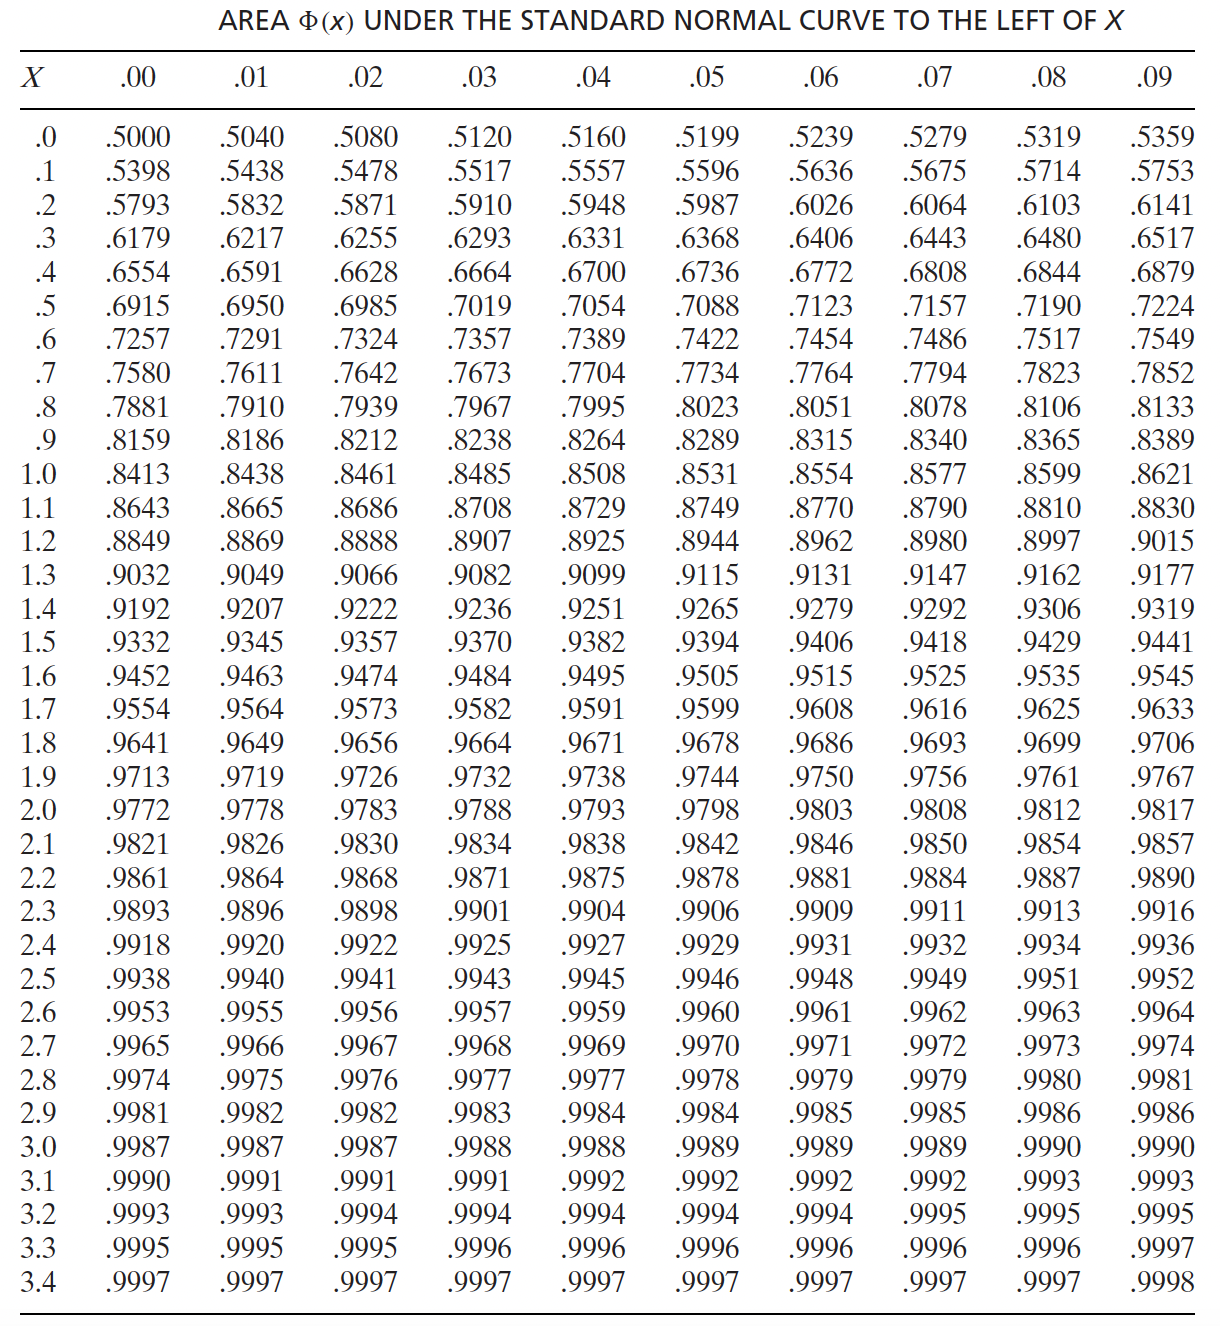
\includegraphics[height=10cm]{images/table1.png}
\\ Table 1
\end{center}

\vspace{0.2cm}

\end{problem}

\begin{problem}{8}
$X$ is a normal random variable with parameters $\mu = 3$ and $\sigma^2 = 9$. Using Table 1, find
\begin{enumerate}[label=(\alph*)]
\item $P(2 < X < 5)$;
\item $P(X > 0)$;
\item $P(|X - 3| > 6)$.
\end{enumerate}
\end{problem}

\begin{problem}{9}
The continuous random variable $X$ is said to have a Weibull distribution with scale parameter $k > 0$ and scale parameter $\sigma > 0$ if the cumulative distribution function of $X$ is
\begin{align*}
    F_X(x) &= 
    \begin{cases}
      1 - e^{-(x/\sigma)^k} & \text{if}\ x \geq 0 \\
      0 & \text{otherwise.}
    \end{cases}
\end{align*}
Find a function $\Phi$ such that the random variable $Y = \Phi(U)$ has the same distribution as $X$, where $U$ is a continuous random variable having a uniform distribution on the interval $[0,1]$.
\end{problem}

\begin{problem}{10}
The continuous random variable $X$ is said to have a pareto distribution with scale parameter $\beta > 0$ and shape parameter $\alpha > 0$ if the probability density function of $X$ is
\begin{align*}
    f_X(x) &= 
    \begin{cases}
      \frac{\alpha \beta^\alpha}{x^{\alpha+1}} & \text{if}\ \beta \leq x < \infty \\
      0 & \text{otherwise.}
    \end{cases}
\end{align*}
Find a function $\Phi$ such that the random variable $Y = \Phi(U)$ has the same distribution as $X$, where $U$ is a continuous random variable having a uniform distribution on the interval $[0,1]$.
\end{problem}

%%%%%%%%%%%%%%%%%%%%%%%%%%%%%%%%%%%%%%%

\newpage

\begin{proof}[Solution: Problem 1]
\text{}\\
\text{}\\
(a) Since $f_X$ is a probability density function, we must have $\int_{-\infty}^\infty f_X(x) dx = 1$, implying that
\begin{align*}
C \int_0^2 (4x-2x^2) dx &= 1\\
C\bigg[2x^2 -\frac{2x^3}{3}\bigg]\bigg|^{x=2}_{x=0} &=  1,
\end{align*}
and hence $C =  \frac{3}{8}$.\\
\text{}\\
(b) $P(X > 1) = \int_1^\infty f_X(x) dx  = \frac{3}{8} \int_1^2 (4x-2x^2) dx = \frac{1}{2}$.
\end{proof}

\vspace{0.2cm}
\begin{proof}[Solution: Problem 2]
\text{}\\
\text{}\\
(a) First find the value of $\lambda$ such that $\int_{-\infty}^\infty f_X(x) dx = 1$.
\begin{align*}
\lambda \int_0^\infty e^{-x/100}dx &=  1\\
-\lambda(100)e^{-x/100} \bigg|^{x=\infty}_{x=0}  &=  1\\
\lambda(100)  &=  1,
\end{align*}
which implies that $\lambda = 1/100$. Hence, 
\begin{align*}
P(50 < X < 150) &= \int_{50}^{150} \frac{1}{100}e^{-x/100}dx\\
&=-e^{-x/100}\bigg|_{50}^{150}\\
&=e^{-1/2} - e^{-3/2}\\
&\approx 0.384
\end{align*}
(b) Similarly, $P(X < 100) = \int_{0}^{100} \frac{1}{100}e^{-x/100}dx = -e^{-x/100}\bigg|_{0}^{100} =1 -e^{-1} \approx 0.633$. In other words, approximately 63.3 percent of the time, a computer will fail before registering 100 hours of use.
\end{proof}

\vspace{0.2cm}
\begin{proof}[Solution: Problem 3]
\text{}\\
\text{}\\
Let $X$ denote the number of minutes past 7 that the passenger arrives at the stop. Since $X$ is a uniform random variable over the interval (0, 30), it follows that the passenger will have to wait less than 5 minutes if (and only if) they arrive between 7:10 and 7:15 or between 7:25 and 7:30. Hence, the desired probability for part (a) is
\begin{equation*}
P(10 < X < 15) + P(25 < X < 30) = \int_{10}^{15}\frac{1}{30}dx + \int_{25}^{30}\frac{1}{30}dx = 1/3.
\end{equation*}
Similarly, they would have to wait more than 10 minutes if they arrive between 7 and 7:05 or between 7:15 and 7:20, so the probability for part (b) is
\begin{equation*}
P(0 < X < 5) + P(15 < X < 20) = \int_{0}^{5}\frac{1}{30}dx + \int_{15}^{20}\frac{1}{30}dx = 1/3.
\end{equation*}
Why are the answers to (a) and (b) the same?
\end{proof}

\vspace{0.2cm}
\begin{proof}[Solution: Problem 4]
\text{}\\
\text{}\\
(a)
The $(100p)$th percentile is the value of $\eta(p)$ that satisfies $p = \int^{\eta(p)}_{-\infty} f_X(x)dx$. It is helpful to first calculate the probability that the total waiting time is less than 5 minutes:
\begin{align*}
P(0 \leq X < 5) &= \int^{5}_{0} \frac{x}{25}dx\\
&= \frac{1}{50}x^2\bigg|^5_0 \\
&= 0.5.
\end{align*}
%and $5 \leq \eta(p) \leq 10$
Therefore, $0 \leq \eta(p) < 5$ when $0 \leq p \leq 0.5$. In this scenario, the $(100p)$th percentile is the value of $\eta(p)$ that satisfies
\begin{align*}
p &= \int^{\eta(p)}_0 \frac{x}{25}dx\\
&= \frac{1}{50}x^2\bigg|^{\eta(p)}_0,
\end{align*}
which is $\eta(p) = \sqrt{50p}$. 
In contrast,  $5 \leq \eta(p) \leq 10$ when $0.5 < p \leq 1$. In this scenario, the $(100p)$th percentile is the value of $\eta(p)$ that satisfies
\begin{align*}
p &= 0.5 + \int^{\eta(p)}_5 \bigg(\frac{2}{5} -\frac{x}{25}\bigg)dx\\
&=  0.5 + \bigg[\frac{2x}{5} -\frac{x^2}{50}\bigg]\bigg|^{\eta(p)}_5\\
&=  0.5 + \bigg(\frac{2\eta(p)}{5} -\frac{\eta(p)^2}{50}\bigg) - \bigg(2 -\frac{1}{2}\bigg).
\end{align*}
Here, the term 0.5 has been added to the right-hand side to account for the probability that the total waiting time is less than 5 minutes. After some algebraic rearranegment, the quadratic formula can be used to solve the equation $\eta(p)^2 - 20\eta(p) + 50p + 50 = 0$. This gives $\eta(p) = 10 - \sqrt{50(1-p)}$. Thus, the expression for the $(100p)$th percentile is
\begin{align*}
    \eta(p) &= 
    \begin{cases}
      \sqrt{50p} & \text{if}\ 0 \leq p \leq 0.5 \\
      10 - \sqrt{50(1-p)} & \text{if}\ 0.5 < p \leq 1.
    \end{cases}
\end{align*}
(b) The median is $\eta(0.5) = 5$.
\end{proof}

\vspace{0.2cm}
\begin{proof}[Solution: Problem 5]
\text{}\\
\text{}\\
The expected value of $e^X$ is
\begin{align*}
\mathbb{E}[e^X] &= \int_{-\infty}^\infty e^X f_X(x) dx\\
&= \int_0^1 e^X dx\\
&= e^X\big|^1_0\\
&= e - 1.
\end{align*}
\end{proof}

\vspace{0.2cm}
\begin{proof}[Solution: Problem 6]
\text{}\\
\text{}\\
(a)
The expected value of $X$ is
\begin{align*}
\mathbb{E}[X] &= \int_0^2 x \bigg(\frac{3x}{8} + \frac{1}{8}\bigg)dx\\
&= \bigg[\frac{x^3}{8} + \frac{x^2}{16}\bigg]\bigg|^2_0\\
&= \frac{5}{4}.
\end{align*}
(b) The variance of $X$ is
\begin{align*}
\mathrm{Var}[X] &= \mathbb{E}[X^2] - \mathbb{E}[X]^2\\
&= \int_0^2 x^2 \bigg(\frac{3x}{8} + \frac{1}{8}\bigg)dx - \bigg(\frac{5}{4}\bigg)^2\\
&= \bigg[\frac{3x^4}{32} + \frac{x^3}{24}\bigg]\bigg|^2_0 - \bigg(\frac{5}{4}\bigg)^2\\
&= \frac{13}{48}.
\end{align*}
\end{proof}

\begin{proof}[Solution: Problem 7]
\text{}\\
\text{}\\
This question can be answered without knowing either $\mu$ or $\sigma$, as long as the distribution is known to be normal; the answer is the same for any normal distribution:
\begin{align*}
P(\text{$X$ is within 1.5 standard deviations from the mean}) &= P(\mu - 1.5 \sigma \leq X \leq \mu + 1.5 \sigma)\\
&= P\bigg(\frac{\mu - 1.5 \sigma - \mu}{\sigma} \leq \frac{X - \mu}{\sigma} \leq \frac{\mu + 1.5 \sigma  - \mu}{\sigma}\bigg)\\
&= P(- 1.5  \leq Z \leq 1.5)\\
&= \Phi(1.5) -  \Phi(-1.5)\\
&= \Phi(1.5) -  [1 - \Phi(1.5)]\\
&\approx 0.8664,
\end{align*}
where $Z = (X - \mu)/\sigma$ is a standard normal random variable with cumulative distribution function $\Phi$.
\end{proof}

\vspace{0.2cm}
\begin{proof}[Solution: Problem 8]
\text{}\\
\text{}\\
(a)
\begin{align*}
P(2 < X < 5) &= P\bigg(\frac{2 - \mu}{\sigma} < \frac{X - \mu}{\sigma} < \frac{5  - \mu}{\sigma}\bigg)\\
&= P\bigg(\frac{2 - 3}{3} < \frac{X - 3}{3} < \frac{5  - 3}{3}\bigg)\\
&= P\bigg(-0.33 < Z < 0.66 \bigg)\\
&= \Phi(0.66) -  \Phi(-0.33)\\
&= \Phi(0.66) -  [1 - \Phi(0.33)]\\
&\approx 0.3747.
\end{align*}
(b)
\begin{align*}
P(X > 0) &= P\bigg(\frac{X - 3}{3} > \frac{0  - 3}{3}\bigg)\\
&= P\bigg(Z > -1 \bigg)\\
&= 1 - P\bigg(Z \leq -1 \bigg)\\
&= 1 - \Phi(-1)\\
&= 1 - [1 - \Phi(1)]\\
&\approx 0.8413.
\end{align*}
(c)
\begin{align*}
P(|X - 3| > 6) &= P(X - 3 > 6)  + P(X - 3 < -6) \\
&= P(X  > 9)  + P(X < -3) \\
&= P\bigg(\frac{X-3}{3}  > \frac{9-3}{3}\bigg)  + P(\frac{X-3}{3} < \frac{-3-3}{3}\bigg)\\
&= P(Z  > 2)  + P(Z < -2)\\
&= 1 - P(Z  \leq 2)  + P(Z < -2)\\
&= 1 - \Phi(2)  + [1-\Phi(2)]\\
&\approx 0.0456.
\end{align*}
\end{proof}

\begin{proof}[Solution: Problem 9]
\text{}\\
\text{}\\
The probability integral transform tells us that $\Phi = F_X^{-1}$, the inverse of the cumulative distribution function. Therefore, to find $\Phi = F_X^{-1}$, set $U = F_X(x)$ and solve for $x$ as a function of $U$. This gives $\Phi  = \sigma(-\log(1-U))^{1/k}$.
\end{proof}

\vspace{0.2cm}
\begin{proof}[Solution: Problem 10]
\text{}\\
\text{}\\
First find the cumulative distribution function $F_X$ and then find its inverse $F_X^{-1}$.
\begin{align*}
F_X(x) &= \int_{-\infty}^x f_X(t) dt\\
&= \int_{-\infty}^x \frac{\alpha \beta^\alpha}{t^{\alpha+1}} dt\\
&= \frac{- \beta^\alpha}{t^{\alpha}} \bigg|_{\beta}^{x}\\
&= 1 - \bigg(\frac{\beta}{x}\bigg)^\alpha.
\end{align*}
To find $\Phi = F_X^{-1}$, set $U = F_X(x)$ and solve for $x$ as a function of $U$. This gives $\Phi = \beta(1- U)^{-1/\alpha}$.
\end{proof}

\end{document}